\chapter{Návrh řešení} % TODO lepe promyslet jak se ujmout teto casti
%popis jednotlivych bloku realizace, s odkazem na blokove schema z Kapitoly 3
Návrh řešení musí brát ohled na primární požadavky, které zařízení musí splňovat, aby byla zajištěna základní funkčnost zařízení. Tyto požadavky byly popsány v části \ref{Technicka specifikace}. Dalšími požadavky na zařízení je miniaturizace vyčítacího rozhraní, tento požadavek stanovuje zadní diplomové práce. V této části budou popsány obecné požadavky na návrh rozhraní a dále v \ref{realizace} bude podrobněji popsán výběr konkrétních součástek a návrh zapojení rozhraní.

\section{Koncept řešení}
Navržený koncept vyčítacího rozhraní je zobrazen na obrázku \ref{fig:navrh_reseni}. Koncept se skládá ze dvou desek plošných spojů (PCB). Toto rozložení bylo navrhnutu s ohledem na požadavky miniaturizace celého zařízení a také s ohledem na variabilitu zařízení. Nebol-li například možnosti připojit k jedné základní desce různé chipboardy, respektive například připojit chipboard, s různým typem senzorové vrstvy detektoru Timepix 2. 
\par Prvním PCB je takzvaná \textit{základní deska}. Na této desce je implementováno většina funkcionalit potřebných pro komunikaci s detektorem Timepix 2. Dále je zde implementována USB komunikace, která slouží pro komunikaci rozhraní přes USB.
\par Druhou deskou plošných spojů je \textit{chipboard}, na této desce se nachází samotný detektor Timepix 2. Dále je zde implementován vysokonapěťový (HV) zdroj a měření teploty.
 
\begin{figure}[h!]
	\centering
	\captionsetup{justification=centering}
	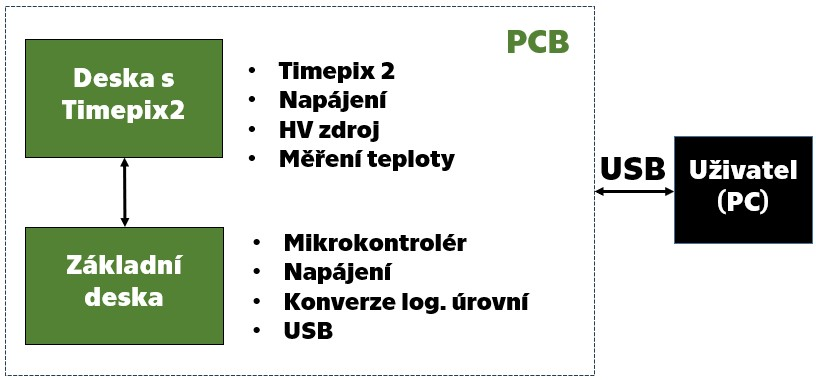
\includegraphics[scale=0.80]{navrh_reseni.jpg}
	\caption{Koncept řešení vyčítacího rozhraní pro detektor Timepix 2} 
	\label{fig:navrh_reseni}
\end{figure}

\subsection{Výpočetní výkon}
\subsubsection{Komunikace s Timepix 2}
Pro komunikaci s Timepix 2 je možné využít sériové, nebo paralelní komunikace, jak již bylo zmíněno v části \ref{Komunikacni rozhrani}. Pro tuto práci uvažujme využití pouze sériové komunikace. Maximální vyčítací rychlost z detektoru Timepix 2 je 100 Mbits/s. S ohledem na tuto maximální rychlost vyčítaní dat z Timepix 2 musí být vybrán vhodný mikrokontrolér pro obsluhu komunikace. 

\subsection{Komunikační rozhraní}
Komunikační rozhraní pro tuto práci bylo zvoleno rozhraní USB konkrétněji standart USB 2.0 High Speed. Tento standart umožňuje komunikovat maximální rychlostí až 480 Mbit/s. S respektem na rychlost vyčítání dat z detektoru Timepix 2 je tato rychlost dostačující. 

\subsection{Napájení}
Pro napájení detektoru Timepix 2 jsou dle \ref{tab:tpx2_napajeni} jsou zapotřebí dvě napájecí napětí. Napájecí zdroje musí být vhodné pro maximální odběr detektoru Timepix 2, která by neměla být větší něž 900 mW. 
\par Dalším potřebným napájením je napájení mikrokontroléru. Toto napájení je závislé na konkrétním typu mikrokontroléru. Detailnější informace o výběru mikrokontroléru budou v části \ref{realizace}.

\subsection{Mechanika}
Návrh rozhraní je rozložen do dvou desek plošných spojů spojenými konektorem. Při návrhu mechanické části zařízení musí být zajištěna mechanické odolnost vůči poškození, možnost se na rozhraní připojit pomocí konektoru a především musí být zajištěn odvod tepla od objektů, které mají největší výkon. Těmito objekty jsou především Timepix 2, mikrokontrolér a napájecí zdroje. 


